\documentclass[a4paper]{article}
\usepackage[margin=25mm]{geometry}
\usepackage{amsmath}
\usepackage{amsfonts}
\usepackage{amssymb}
\usepackage{graphicx}
\pagenumbering{gobble}
\usepackage{verbatim}
\usepackage[utf8]{inputenc}
\usepackage[french,english]{babel}
\usepackage{tikz}
\usepackage{xcolor}

\newtheorem{theorem}{Th\'eor\`eme}[subsection]
\newtheorem{proposition}{Proposition}[subsection]
\newtheorem{definition}{D\'efinition}[subsection]

\newtheorem{lemma}{Lemme}[subsection]
\newtheorem{model}{Mod\`ele}[subsection]
\newtheorem{algorithm}{Algorithme}[subsection]
\newtheorem{problem}{Probl\`eme}[subsection]
\newtheorem{remark}{Remarque}[subsection]

%\newcommand{\Id}{\mathbf{Id}}
%\newcommand{\ie}{$i. e.\ $}
%\newcommand{\eg}{$e. g.\ $}
%\newcommand{\st}{ such that }
%\newcommand{\Div}{\mbox{div }}
%\newcommand{\Curl}{\mbox{curl }}

% Keywords command
\providecommand{\keywords}[1]
{
  \small	
  \textbf{\textit{Keywords---}} #1
}

\title{Titre du rapport}

\author{Premier Auteur$^{1}$, Second Auteur$^{2}$  \\
        \small $^{1}$L3 LDD Informatique, Mathématiques, Université Paris-Saclay, 91405 Orsay, France \\
        \small $^{2}$L3 LDD Mathématiques, Physique, Université Paris-Saclay, 91405 Orsay, France \\
}

\date{} % Comment this line to show today's date


\makeindex      

%%%%%%%%%%%%%%%%%%%%%%%%%%%%%%
\begin{document}
\selectlanguage{french} 

\maketitle

\begin{tikzpicture}[overlay,yshift=5cm, xshift=13.4cm]
  \pgftext{
\includegraphics[width=90pt]{logo-ups.png}}
\end{tikzpicture}

\begin{abstract}
{\color{blue}Résumé en français...}
Lorem ipsum dolor sit amet, consectetur adipiscing elit. Vestibulum pretium libero non odio tincidunt semper. Vivamus sollicitudin egestas mattis. Sed vitae risus vel ex tincidunt molestie nec vel leo. Vestibulum ante ipsum primis in faucibus orci luctus et ultrices posuere cubilia Curae; Maecenas quis massa tincidunt, faucibus magna non, fringilla sapien. In ullamcorper justo a scelerisque egestas. Ut maximus, elit a rutrum viverra, lectus sapien varius est, vel tempor neque mi et augue. Fusce ornare venenatis nunc nec feugiat. Proin a enim mauris. Mauris dignissim vulputate erat, vitae cursus risus elementum at. Cras luctus pharetra congue. Aliquam id est dictum, finibus ligula sed, tempus arcu. 
\end{abstract} 
\hspace{10pt}

\selectlanguage{english} 
\begin{abstract}
{\color{blue}Abstract in English... }
Lorem ipsum dolor sit amet, consectetur adipiscing elit. Vestibulum pretium libero non odio tincidunt semper. Vivamus sollicitudin egestas mattis. Sed vitae risus vel ex tincidunt molestie nec vel leo. Vestibulum ante ipsum primis in faucibus orci luctus et ultrices posuere cubilia Curae; Maecenas quis massa tincidunt, faucibus magna non, fringilla sapien. In ullamcorper justo a scelerisque egestas. Ut maximus, elit a rutrum viverra, lectus sapien varius est, vel tempor neque mi et augue. Fusce ornare venenatis nunc nec feugiat. Proin a enim mauris. Mauris dignissim vulputate erat, vitae cursus risus elementum at. Cras luctus pharetra congue. Aliquam id est dictum, finibus ligula sed, tempus arcu. 
\end{abstract}
\selectlanguage{french}


%TC:ignore
\keywords{mot clé; mot clé; mot clé}

\clearpage

\section{Introduction}

Aenean tellus orci, accumsan $i$ nec neque at, vestibulum eleifend elit \cite{helbing09,SchadCA09} ({\color{blue}bien cité dans le texte de l'article toute référence présente dans la bibliographie}) Sed luctus enim dui, in fermentum $j$ dui pharetra at. Fusce vel nisl et diam feugiat porttitor et at libero. Maecenas scelerisque varius mauris non euismod. Nulla eget cursus leo. Integer interdum lacus vel ligula maximus, at feugiat orci porttitor. Suspendisse egestas, lorem a \index{elementum} lobortis, tellus mauris hendrerit nunc, sed vestibulum mi velit quis risus. Mauris gravida mi et ullamcorper blandit. Aenean lacinia, quam id tempus interdum, massa orci rhoncus turpis, eu finibus nisi lectus id sem. Vivamus ut mauris sed diam porta viverra sit amet quis risus (\cite{Zuriguel09}).

Nam id ornare dolor. Nulla metus enim, venenatis vel dui ac, accumsan vehicula est. Suspendisse luctus eros et velit eleifend, nec finibus ante rutrum. Interdum et malesuada fames ac ante ipsum primis  {\em systemic} in faucibus. Vivamus tempor lorem turpis, nec venenatis turpis venenatis nec. Integer hendrerit at mi nec aliquet. Vestibulum auctor arcu scelerisque lacus rhoncus ornare. Vivamus convallis libero nulla, vitae ullamcorper mauris venenatis nec. Donec elementum ligula non tortor \index{pellentesque} finibus.

Vestibulum mauris odio, scelerisque ut nisi ut, tincidunt maximus eros. Fusce tempor ex non mi commodo consectetur. Sed sit amet massa id elit commodo bibendum. Nunc id neque tempus erat tempus dictum. Fusce mi leo, hendrerit in egestas sed, faucibus vel ex. In hac habitasse platea dictumst. Vivamus eget odio arcu. Ut finibus et lacus ac interdum. Donec consectetur dolor neque, vel condimentum nunc varius nec. Mauris sapien dolor, aliquam nec vulputate at, fermentum vel nulla. Orci varius natoque penatibus et magnis dis parturient montes, nascetur ridiculus mus. Class aptent taciti sociosqu ad litora torquent per conubia nostra, per inceptos himenaeos. Nam posuere vulputate vestibulum.

\section{Première section}

Integer iaculis vitae nisi mollis congue. Cras sed facilisis tortor. Aliquam quis neque ipsum. Proin et accumsan arcu. Donec sit amet nibh lacus. Vestibulum mattis arcu sed ante \index{vestibulum} condimentum. Nunc auctor ligula vel velit finibus imperdiet. Cras consequat ipsum quis rhoncus consequat. Etiam luctus purus turpis, quis tempor massa posuere non. Donec vitae $\Phi$ ex in ligula ultricies feugiat. Sed urna sem, rutrum at tempus vel, mollis vel magna. Etiam ex est, pulvinar et risus at, facilisis efficitur turpis. Etiam egestas est a erat elementum, vitae porta lectus finibus. Donec ac consequat sapien. Aenean sed eros a est blandit dictum.\\
{\color{blue}Equation numérotée pouvant être citée (\ref{eq:eq1}) : }
\begin{equation}
\label{eq:eq1}
( a + b )^2 = a^2 + b^2 + 2 a b. 
\end{equation}

\noindent{\color{blue}Système d'équations : }
\begin{eqnarray}
\label{eq:eq2}
( a + b )^2 &=& a^2 + b^2 + 2 a b,\\
( a - b )^2 &=& a^2 + b^2 - 2 a b.
\end{eqnarray}



Quisque in dui porttitor, finibus lacus quis, pretium dui. Nullam vitae augue ligula. Nulla vel nisl tincidunt, ullamcorper enim nec, sollicitudin justo. Praesent vitae ex elit. Sed placerat velit a lectus fringilla, in tempor lorem efficitur. Maecenas mattis  $n = 1,\dots,m_i$, tellus ipsum, a laoreet quam aliquam eu. Donec eu interdum lectus. Morbi suscipit nibh (\ref{eq:eq1})sed enim interdum, eget aliquam odio ullamcorper. Sed at mauris maximus, mollis mi ut, dapibus mauris. Morbi efficitur ultricies massa, et vulputate est pellentesque nec $\alpha_i^n$. Curabitur rutrum ullamcorper efficitur. Curabitur vestibulum consequat orci quis dapibus. Ut a ullamcorper tellus. Proin fermentum malesuada dui ac mollis. Mauris volutpat finibus lacus et placerat. \\
{\color{blue}Equation non numérotée : }
\begin{equation*}
( a - b )^2 = a^2 + b^2 - 2 a b. 
\end{equation*}

\section{Seconde section}

\subsection{Première sous-section}

Curabitur nulla libero, viverra at tempus vitae, ornare ac metus. Nullam sed imperdiet erat, a vestibulum arcu. Sed non nisi cursus, sagittis libero in, pellentesque est. Pellentesque habitant morbi tristique senectus et netus et malesuada fames ac turpis egestas. Interdum et malesuada fames ac ante ipsum primis in faucibus. Sed congue turpis ligula, et tristique neque scelerisque sit amet. Vivamus neque est, pharetra eu libero at, tincidunt feugiat augue.

\begin{definition}
On appelle... 
\end{definition}


\subsection{Seconde sous-section}

\begin{theorem}
Soit une fonction $\Phi$... 
\end{theorem}

\begin{lemma}
Soit $x \in \mathbf{R}$,...
\end{lemma}

\begin{remark}
On remarque que...
\end{remark}

Morbi mollis sapien nisi, non fringilla felis placerat vitae. Donec ac enim justo. Cras placerat purus vel ex volutpat, eget placerat lorem fermentum. Duis quam risus, eleifend quis iaculis eu, efficitur at nisl. Pellentesque pharetra dui nisi, sit amet sodales mi hendrerit nec. Nullam et gravida lorem, ut faucibus dolor. Mauris bibendum pulvinar tortor, eget consequat nulla luctus eget.

\begin{figure}[t]
 \begin{center}
   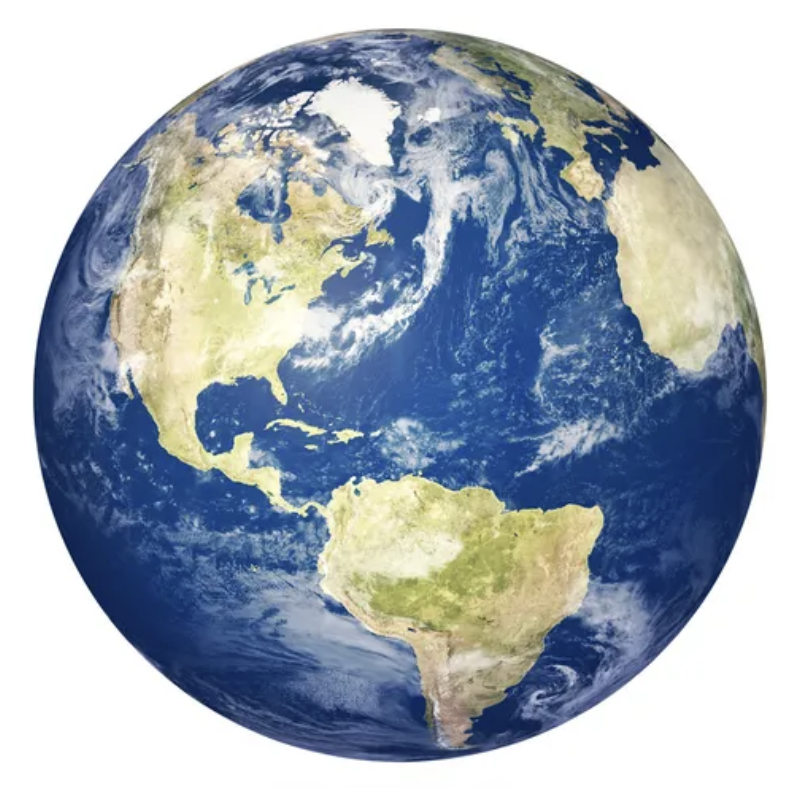
\includegraphics[width=0.295\linewidth]{terre.png}

 \end{center}
 \caption{La Terre}
\label{fig:fig1}
\end{figure}

{\color{blue}Bien penser à citer et à commenter toutes les figures du texte : (Figure \ref{fig:fig1})}
Quisque in dui porttitor, finibus lacus quis, pretium dui. Nullam vitae augue ligula. Nulla vel nisl tincidunt, ullamcorper enim nec, sollicitudin justo. Praesent vitae ex elit. Sed placerat velit a lectus fringilla, in tempor lorem efficitur. Maecenas mattis tellus ipsum, a laoreet quam aliquam eu. Donec eu interdum lectus. Morbi suscipit nibh sed enim interdum, eget aliquam odio ullamcorper. Sed at 

\section{Conclusion}

Curabitur nulla libero, viverra at tempus vitae, ornare ac metus. Nullam sed imperdiet erat, a vestibulum arcu. Sed non nisi cursus, sagittis libero in, pellentesque est. Pellentesque habitant morbi tristique senectus et netus et malesuada fames ac turpis egestas. Interdum et malesuada fames ac ante ipsum primis in faucibus. Sed congue turpis ligula, et tristique neque scelerisque sit amet. Vivamus neque est, pharetra eu libero at, tincidunt feugiat augue.

\section*{Remerciements}

Les auteurs de ce document remercient vivement... 


\begin{thebibliography}{99}

\bibitem{helbing09}
D. Helbing,  
A. Johansson,  
Pedestrian, Crowd and Evacuation Dynamics, 
\emph{Encyclopedia of Complexity and Systems Science},
pp. 6476--6495, Springer New York.

\bibitem{SchadCA09}
A. Schadschneider, A. Seyfried, Empirical results for pedestrian dynamics and their implications for cellular automata models,
in``Pedestrian Behavior'', Ed.: H. Timmermans, Emerald, p. 27 (2009).

\bibitem{Zuriguel09}
I. Zuriguel, J.     Olivares, J.M.   Pastor, C.  Mart\'in-G\'omez,  L.M. Ferrer, J.J.  Ramos, A. Garcimart\'in, 
Effect of obstacle position in the flow of sheep through a narrow door, 
\emph{Phys. Rev. E},  94.

\end{thebibliography}




\end{document}
